% ------------------------------------------------------------------------------------
% Competitor comparison.
% Figures: figures/competitor/fig_cmp_{strips,context_growth,pareto}.pdf
%   fig_cmp_strips = 3-panel dashboard (effect | speed | cost).
% Data: competitor_comparison/metrics.json
% All numbers + figures regenerable via: python paper/arxiv_2026/competitor_comparison/make_figures.py
% ------------------------------------------------------------------------------------

\section{Comparison with Open-Source Accumulating-Context Agents}
\label{sec:competitors}

The submitted version compared against external calibration anchors only. Here we add a
direct, same-testbed \emph{operational} comparison against the two open-source StS2 agents
that could be run faithfully end-to-end: \textbf{STS2MCP}~\citep{sts2mcp-2026} and
\textbf{CharTyr}~\citep{chartyr-sts2-2026}. Both follow the dominant agent-loop design our
contract argues against: a single accumulating chat transcript, re-sent (and grown) on
every decision. We stress at the outset that this is a comparison of \emph{shipped systems},
not a controlled ablation of the memory contract: the competitors differ from our agent in
game patch, routing, thinking effort, decision batching, and prompt cadence as well as in
the contract, so the gaps below characterize the current state of practice rather than
isolating boundedness as the cause.

\paragraph{Faithful replication.}
Each competitor runs its \emph{author-intended} configuration: the author's own mod build
(minimal load-compatibility patches only; zero agent-logic changes), the author's own MCP
server, and the author's own skill/strategy documents as the system prompt, driven through
their tool interface. A leak audit over the captured requests confirms no content from our
project enters their context. Exactly one mod is loaded at a time, and every game is a
fresh Silent $A_0$ run on the same machine and the same v0.103.x line of the game: our
cells ran on v0.103.1; a minor game patch (v0.103.3, 2026-05-30) landed between the two
batches, so competitor runs used v0.103.3 (their mods compile against the v0.103.1-pinned
reference and load cleanly on v0.103.3; our own stack re-verified on v0.103.3). All strategic
decisions for every agent run on \texttt{gemini-3.1-pro-preview}; our agent additionally
routes trivial decisions to a flash-lite fast tier and sets explicit thinking effort,
while competitors run at the provider default with no thinking parameter (their intended
setup). The denominator is completed games --- harness failures are re-run, never counted
as losses --- and every run ended in a natural in-game terminal, none at the decision cap.
All raw prompts, responses, token usage, and per-step game state are released
(released with the data archive).

\paragraph{Effect.}
Figure~\ref{fig:cmp-dashboard}(a) shows run scores ($s = 100$ if victory else
$\mathrm{floor} + (52/3)\cdot\mathrm{bosses}$, \S\ref{sec:testbed}). Both accumulating
agents collapse at $A_0$: STS2MCP wins $0/5$ (mean floor 17.6; one Act-1 boss cleared
across five runs), CharTyr wins $0/5$ (mean floor 5.6; its frequent
\texttt{invalid\_action} interface errors compound into early deaths --- a property of the
agent under test, faithfully reproduced\footnote{CharTyr outcomes for runs 2--5 are
inferred from terminal floors 5--6 plus the absence of any victory flag anywhere in the
captures; run 1's defeat is confirmed by its captured structured
\texttt{game\_over.is\_victory=false}. All captures are released for audit.}). Our
\texttt{full-frozen} cell wins $6/10$ (mean score 82.1) and even \texttt{baseline-strict}
--- our harness with the bounded contract but no learned stores --- wins $3/10$ (70.4),
so the gap is not explained by harness quality alone.

\paragraph{Speed and cost.}
Figure~\ref{fig:cmp-dashboard}(b,c) and Figures~\ref{fig:cmp-growth}--\ref{fig:cmp-pareto}
quantify the operational gap.
Per floor reached, the accumulating agents need $\sim$4$\times$ the wall clock
(9.9\,/\,8.5 vs.\ 2.3 minutes; 96\% of their wall-clock is provider-reported LLM latency,
so the gap is not harness pacing). Per score point, they spend $66$--$90\times$ more
\emph{fresh} (non-cached) LLM tokens; under raw ingested context the multiplier exceeds
$450\times$, and even pricing every recorded action of ours as a full strategic call
(an intentionally absurd upper bound) leaves $\geq 7\times$. Part of this gap is decision
batching --- one strategic call drives multiple actions in our agent, while the
competitors call the LLM once per action by design --- which we report as a property of
the memory-architecture package rather than of the backbone.
Figure~\ref{fig:cmp-growth} shows the mechanism: their per-call prompt grows from
$\sim$9k to $500$k tokens within a single run (trimming caps message \emph{count}, but
late-game states grow each message), while the bounded contract holds the strategic user
message flat at a $\sim$5k median.

\begin{figure}[t]
  \centering
  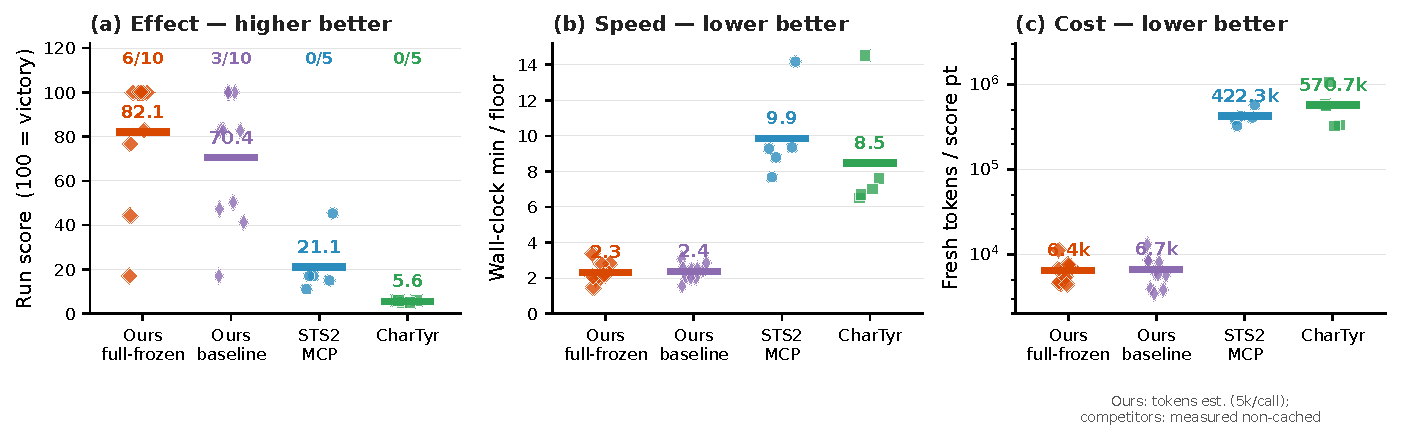
\includegraphics[width=\linewidth]{figures/competitor/fig_cmp_strips.pdf}
  \caption{Competitor comparison at $A_0$ (The Silent), per run; horizontal bars are
  per-cell means. \textbf{(a) Effect}: run score ($s=100$ if victory else
  $\mathrm{floor}+(52/3)\cdot\mathrm{bosses}$), with win counts above each column.
  \textbf{(b) Speed}: wall-clock minutes per floor reached (96\% of competitor wall-clock
  is provider-reported LLM latency; fixed inter-action delays slightly favor competitors,
  0.5s vs.\ our 0.6s; our durations exclude postrun). \textbf{(c) Cost}: fresh (non-cached)
  LLM tokens per score point (log). Competitor usage is exact provider-reported tokens with
  cache hits removed (90\%\,/\,82\% of their prompt tokens were cached); ours follows the
  paper's Fig.~3 convention ($\sim$5k strategic user-message tokens $\times$
  \texttt{llm\_calls}), excluding the cached system prefix, completions, retries, and
  fast-tier calls. \texttt{full-frozen}/\texttt{baseline-strict} are the Table~2 cells
  ($N{=}10$, frozen stores at SHA \texttt{1888a62}); competitors $N{=}5$. Under the
  intentionally absurd upper bound pricing \emph{every} recorded action as a full strategic
  call, our cells move to 55k\,/\,58k tokens per point --- the gap remains $\geq 7\times$.}
  \label{fig:cmp-dashboard}
\end{figure}

\begin{figure}[t]
  \centering
  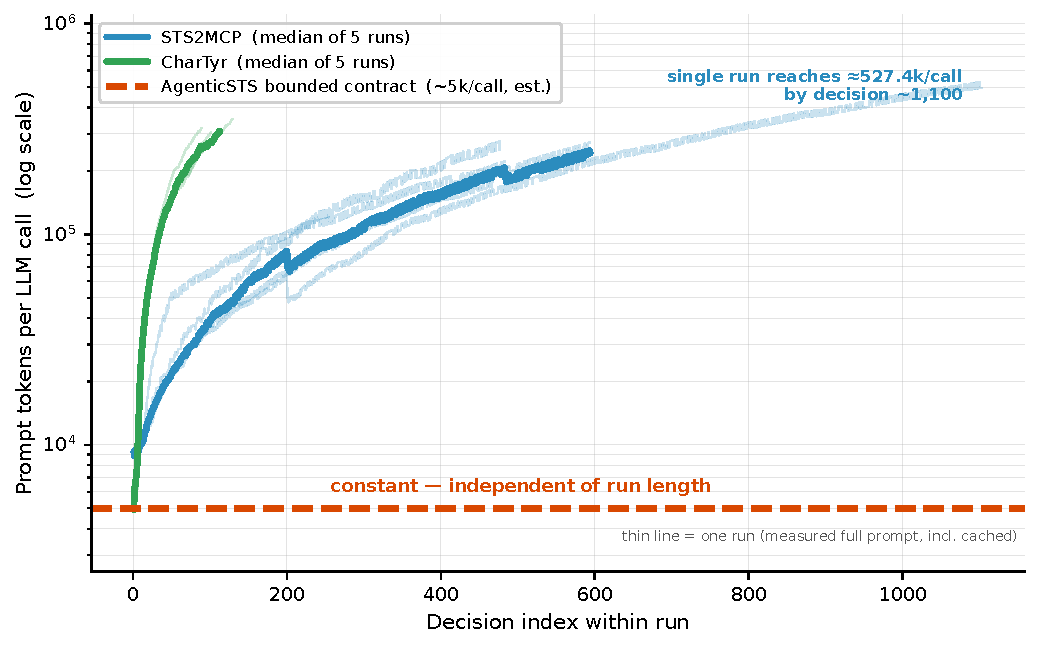
\includegraphics[width=\linewidth]{figures/competitor/fig_cmp_context_growth.pdf}
  \caption{The mechanism: per-call prompt size over a run. Thin lines are individual runs
  (measured full prompts, including cached tokens --- caching changes billing, not what the
  model attends to); bold lines are per-competitor medians. The worst single STS2MCP run
  reaches $\sim$500k tokens per call by decision $\sim$1100. The dashed line is our bounded
  contract's strategic user-message median ($\sim$5k, estimate; constant cached system prefix
  excluded; $x$-extent not comparable --- our runs make $\sim$100 strategic calls).}
  \label{fig:cmp-growth}
\end{figure}

\begin{figure}[t]
  \centering
  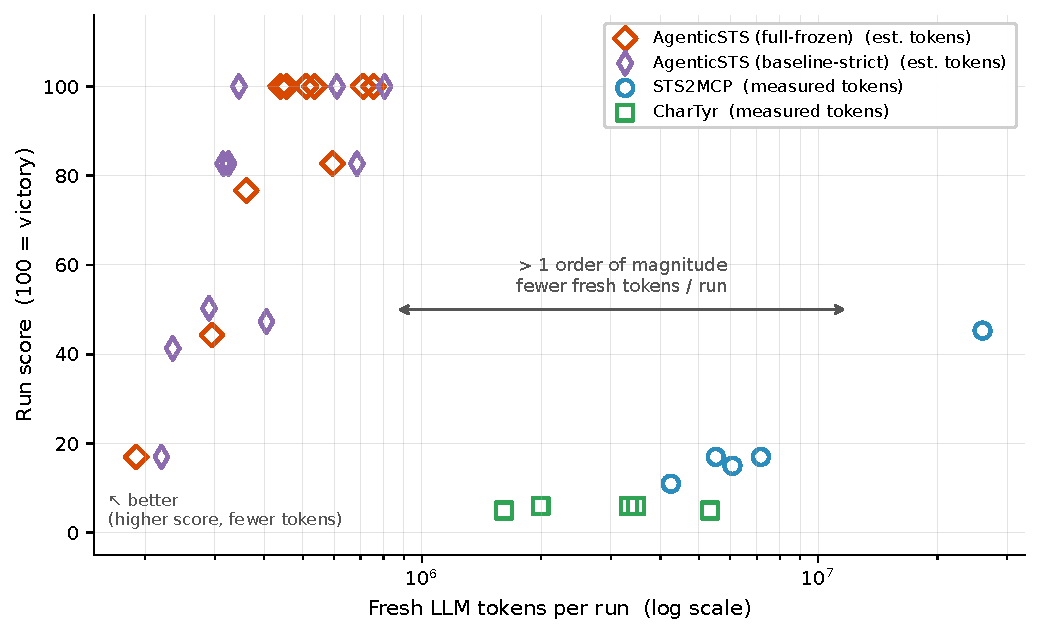
\includegraphics[width=\linewidth]{figures/competitor/fig_cmp_pareto.pdf}
  \caption{Cost--effect frontier: run score vs.\ fresh LLM tokens per run (log). Hollow
  diamonds: our cells (tokens estimated, 5k/call convention); circles/squares: measured
  competitor usage. The empty band between the clusters spans more than an order of
  magnitude.}
  \label{fig:cmp-pareto}
\end{figure}

\paragraph{What this comparison does and does not show.}
It does not show that accumulating context can never win StS2 --- both competitors are
community projects, not tuned baselines, and CharTyr's losses are partly interface
errors. It does show that the two publicly available transcript-accumulating agents,
run faithfully on the same backbone, game line, character, and ascension, with the
denominator rules of our own evaluation, fall far below even our no-store bounded
baseline while consuming one to two orders of magnitude more tokens per point of
progress. A matched same-codebase accumulating-context cell would isolate the
contract variable itself; we leave that controlled comparison to follow-up work,
and this release is organized to support it. The present section establishes the
external state of practice under disclosed operational differences.
